\section{The Development of the mobile Client}
\subsection{Preconditions}
\subsubsection{Norms for mobile Apps}
As already mentioned, ePill is currently only used in Germany, therefor we will focus on laws applicable in Germany. These laws are namely the \TKGns, the \TMGns, the \REG as well as the \DPA of \NRWns. The \TKG and \TMG are laws by state, whereas \REG is an european directive, specified by the respective Member States. 
\\
German federal states have their own \DPAsns. In this thesis we will focus on the \DPA of \NRW as ePill is located in \NRWns.
\\
\\
As the topmost layer of laws, the \REG defines more general directives. Article 4 defines national law applicable, if the natural or legal person, the controller\footnote{cf. \cite{TheEuropeanParliamentandtheCounciloftheEuropeanUnion.24.10.1995}, Article 2, (d)}, is located on a Member State's territory\footnote{cf. \cite{TheEuropeanParliamentandtheCounciloftheEuropeanUnion.24.10.1995}, Article 4, 1., (a) and (b)} or if any of the processing takes place on a Member State's territory\footnote{cf. \cite{TheEuropeanParliamentandtheCounciloftheEuropeanUnion.24.10.1995}, Article 4, 1., (c)}. Furthermore it is required, that the controller asks the user to consent to the use and collection of data\footnote{cf. \cite{TheEuropeanParliamentandtheCounciloftheEuropeanUnion.24.10.1995}, Article 7, (a)}, explicitly "data concerning health and sex life"\footnote{\cite{TheEuropeanParliamentandtheCounciloftheEuropeanUnion.24.10.1995}, Article 8, 1.} shall not be processed. Only if the user consents explicitly\footnote{cf. \cite{TheEuropeanParliamentandtheCounciloftheEuropeanUnion.24.10.1995}, Article 8, 2., (a)} or if the processing is done by a healthcare professional under national law and for preventive medicine, medical diagnosis or treatment or for the management of health-care services\footnote{cf. \cite{TheEuropeanParliamentandtheCounciloftheEuropeanUnion.24.10.1995}, Article 8, 3.}. 
\\
\\
This is refined by the the \TMGns. § 13, section (1) states, that the controller has to inform the user in a commonly understandable manner about the data which is collected and the form of processing of this data\footnote{cf. \cite{BundesregierungderBundesrepublikDeutschland.01.03.2007}, § 13, section (1)}. For a legal consent, the controller has to ensure, that the user is aware of his consent, that the consent is minuted, that the content of the consent is always available to the user and that the user can revoke his consent\footnote{cf. \cite{BundesregierungderBundesrepublikDeutschland.01.03.2007}, § 13, section (2)}.
\\
§§ 91, 93 and 94 of the \TKG states the same laws\footnote{cf. \cite{BundesregierungderBundesrepublikDeutschland.01.08.1996}, Section 2, §§ 91, 93, 94}.
\\
Also the \DPA of \NRW constitutes the same laws\footnote{cf. \cite{DerInnenministerdesLandesNordrheinWestfalen.09.06.2000}, Section 1, §§ 2, 4, 5} with the only restrictions, that its scope is limited to \NRWns.
\\
\\
Therefor ePill should explicitly inform the user that no data is stored and only anonymized transacted to find matching results, to comply with the stated laws.

\subsubsection{Best Practices}
The World Wide Web Consortium (W3C) has published a document in 2008 which states the basic best practices for developing for the mobile web. This document states 60 best practices, which shall ensure a minimum quality level for mobile web applications. These best practices emphasize the need of regard of the device's capabilities and supported technologies\footnote{cf. \cite{WorldWideWebConsortium.2008}, e.g. 2., 11., 21., 42.}. 
\\
This document focuses on mobile web development\footnote{cf. \cite{WorldWideWebConsortium.2008}, Abstract}, which has of course differences to native app development (e.g. the usage of frames and the accessibility of the device's specific features), most of the best practices are applicable in both development environments.
\\
\\
For this specific project, which does not need more specific device capabilities, like positioning and navigation features, we can focus on best practices related to the user interface, input and navigation methods as well as general best practices. Depending on the framework chosen, some of the best practices are already dealt with by the framework or at least supported. E.g. a thematic consistency\footnote{cf. \cite{WorldWideWebConsortium.2008}, 1.} is provided by native apps by default and by frameworks such as the TouchKit for Vaadin as well. Although they can be overridden, they provide a consistent theme. \cite{Wessels.2011} support the importance of a consistent appearance, also in comparison to a desktop application, if existent\footnote{cf. \cite{Wessels.2011}, p. 2}. \cite{Lica.2010} further limits this to specific elements and points out, that mobile apps should provide just enough functionality to be useful and should not replicate the desktop optimized website\footnote{cf. \cite{Lica.2010}, p. 66}.
\\
Other best practices like utilizing a navigation bar at the page's top\footnote{cf. \cite{WorldWideWebConsortium.2008}, 8.} for the main navigation have already become a standard across different platforms and frameworks.
\\
\\
Best practices which are mainly determined by implementations of the developer, like the usage of colors\footnote{cf. \cite{WorldWideWebConsortium.2008}, 26., 27} or the chosen input methods\footnote{cf.\cite{WorldWideWebConsortium.2008}, 55., 56., 57.} are often supported by the different platforms or frameworks but cannot be guaranteed by those. Even if different input methods like a number pad for numeric inputs are provided by the framework or platform they still need to be adapted and utilized by the developer to act in line with the best practices.
\\
\\
\cite{WorldWideWebConsortium.2008} furthermore specifies a "Default Delivery Context"\footnote{cf. \cite{WorldWideWebConsortium.2008}, 3.7 Default Delivery Context}, which defines the minimal capabilities for mobile devices which should be supported. \ref{tab:DefaultDeliveryContext} illustrates the minimal capabilities suggested by W3C.
\\
Nowadays it will be hard to match all of the requirements. E.g. a total maximum page weight of 20 kilobytes corresponds to the average file size of a 200 by 120 pixel JPEG-compressed file is about 10 kilobytes\footnote{Tested with 60\% compression rate and a random photograph} and two images would already exceed the maximum page weight. With mobile devices like a Samsung Galaxy S3 which has a minimum of 720 pixel wide display, 120 pixels are far too less.
\\
Also nearly any mobile browser supports client side scripting (e.g. JavaScript). For more detail, \url{http://caniuse.com} has compatibility lists of different browser features for nearly any browser. The parsing of JavaScript Object Notation (JSON) for example is supported by 93.41\% of all mobile browsers\footnote{cf. \url{http://caniuse.com/\#cats=JS_API}, JSON parsing}.
\begin{table}[!tb]
    \center
    \begin{tabular}{l | p{21.5em}}
        \textbf{Parameter} & \textbf{Value} \\
        \hline
        Usable Screen Width & 120px \\
        \hline
        Markup Language Support & XHTML Basic 1.1 delivered with content type application/xhtml+xml. \\
        \hline
        Character Encoding & UTF-8 \\
        \hline
        Image Format Support & JPEG. \\
        & GIF 89a. \\
        \hline
        Maximum Total Page Weight & 20 kilobytes. \\
        \hline
        Colors & 256 Colors, minimum. \\
        \hline
        Style Sheet Support & CSS Level 1. In addition, CSS Level 2 @media rule together with the handheld and all media types. \\
        \hline
        HTTP & HTTP/1.0 or more recent. \\
        \hline
        Script & No support for client side scripting. \\
    \end{tabular}
    \caption[Mobile Default Delivery Context]{Default Delivery Context\footnotemark}
    \label{tab:DefaultDeliveryContext}
\end{table}
\footnotetext{cf. \cite{WorldWideWebConsortium.2008}, 3.7 Default Delivery Context}
\\
Nevertheless, minimizing the total page size is still a concern. \cite{Wessels.2011} points out, that smaller pages lead to faster load times and therefor provide a more efficient experience for the user\footnote{cf. \cite{Wessels.2011}, p. 1}. \cite{Nicolaou.2013} suggests different approaches to reduce page size as well as load time: Scripts and markup should be minified\footnote{cf. \cite{Nicolaou.2013}, p. 49} and included inline\footnote{cf. \cite{Nicolaou.2013}, p. 50} where it is possible. Preloading components and reducing DNS lookups can also result in a faster user experience\footnote{cf. \cite{Nicolaou.2013}, pp. 48, 49}.
\\
Generally, \cite{Nicolaou.2013} recommends using a Content Delivery System (CDN), putting style sheets at the page's top and scripts at the bottom and using resized images rather than scaling them via HTML or CSS\footnote{cf. \cite{Nicolaou.2013}, pp. 49, 50}.
\\
\\
A study by \cite{Dahanayake.2010} came to the result, that 71\% of all responding web developers knew about the best practices, but only 11\% said, that they understand these, 56\% have a vague understanding and 33\% do not understand the best practices \footnote{cf. \cite{Dahanayake.2010}, p. 85}.
\\
\\
\cite{AyobNurulZakiahbinti.2009} adjusted and combined four different guidelines for application development, namely Shneiderman’s Golden Rules of Interface Design, Seven Usability Guideline for Mobile Device (Abid Warsi, 2007), Human-Centred Design (ISO Standard 13407) and Mobile Web Best Practices 1.0 (W3C). From those guidelines, they developed the Three Layers Design Guideline for Mobile Application\footnote{cf. \cite{AyobNurulZakiahbinti.2009}, p. 430}. This guideline consists of three phases, which themselves represent different contexts, namely analysis (and the context of use), design (the context of medium) and testing (the context of evaluation). \ref{tab:ThreeLayersDesignGuideline} illustrates this guideline.
\\
\\
This thesis will follow the Three Layers Design Guideline, as it is the latest guideline and combines multiple approved other guidelines. The third phase will likely be shortened due to the temporal restrictions for this thesis. The exact process we followed will be outlined in the following subsections \ref{subsec:Analysis} \nameref{subsec:Analysis}, \ref{subsec:Planning} \nameref{subsec:Planning}, \ref{subsec:Implementation} \nameref{subsec:Implementation} and \ref{subsec:Validation} \nameref{subsec:Validation} and the experiences made will be discussed in section \ref{sec:LessonsLearned} \nameref{sec:LessonsLearned}.

\begin{table}[!htb]
    \center
    \begin{tabular}{c | c | p{23.5em}}
        \multicolumn{2}{c | }{\textbf{Phase}} & \textbf{Context of Use and Activities} \\
        \hline
        1 & Analysis & \textbf{Use}: Specify user and organizational requirements \\
        \cline{3-3}
        & & 
            \begin{enumerate}
                \item Identify and document user’s tasks
                \item Identify and document organizational environment
                \item Define the use of the system
            \end{enumerate} 
        \\
        \hline
        2 & Design & \textbf{Medium}: Produce design solution \\
        \cline{3-3}
        & & 
            \begin{enumerate}
                \item Enable frequent users to use shortcuts
                \item Offer informative feedback
                \item Consistency
                \item Reversal of actions
                \item Error prevention and simple error handling
                \item Reduce short-term memory load
                \item Design for multiple and dynamic contexts
                \item Design for small devices
                \item Design for speed and recovery
                \item Design for “top-down” interaction
                \item Allow for personalization
                \item Don't repeat the navigation on every page
                \item Clearly distinguish selected items
            \end{enumerate}
        \\
        \hline
        3 & Testing & \textbf{Evaluation}: Evaluate design against user requirements \\
        \cline{3-3}
        & & 
            \begin{enumerate}
                \item Quick approach
                \item Usability testing
                \item Field studies
                \item Predictive evaluation
            \end{enumerate}
        \\
    \end{tabular}
    \caption[Three Layers Design Guideline for Mobile Application]{Three Layers Design Guideline for Mobile Application\footnotemark}
    \label{tab:ThreeLayersDesignGuideline}
\end{table}
\footnotetext{cf. \cite{AyobNurulZakiahbinti.2009}, p. 430, Table IV}

\subsubsection{Internal requirements}
For developing a mobile frontend for ePill, it is important to us, that the main functionality of the web client is optimized but not reduced. Therefor a good user interface is indispensable. All functionality should be accessible easily and without confusion for the user. Interactive elements like buttons should be visibly salient and have an immediate response to reduce the user's uncertainty. The general design, the color scheme and the fonts should be used in line with the web application to improve the recognition value. 
\\
Another top priority is the accessibility of the app for as many users as possible. Therefor it is needed to provide a cross-platform app to be accessible for as many mobile platforms as possible and to have an intuitive user interface which also enables e.g. elderly people to use it efficiently.
\\
\\
Modularity and flexibility is another important factor. ePill is designed to be flexible and scalable and the mobile client should incorporate the same idea. E.g. a scanning of barcodes on the packaging of pharmaceuticals could be implemented on a later stage to even further ease the use and increase the effectiveness.
\subsection{Analysis}
\label{subsec:Analysis}
\subsubsection{Assignment of a mHealth App Category}
The mobile app does not differ from the web application in terms of privacy risks, content or connectivity. The mobile app aims to provide the same main functionality as the web application optimized for mobile devices. Therefor it also belongs to the same connectivity category, the medical connectivity, as the web application. Also no data is stored on the device and no additional information is sent to the server. 
\\
We plan to implement every request to the server to be optimized for SSL-encryption as soon as the server is capable of accepting and responding with SSL-encryption. 
\\
\\
Therefor we would suggest to categorize the ePill mobile application as a low privacy risk, drug- and safety-related medical connectivity mHealth application and should be categorized similar to the web application. 
\\
Possible future features might change the classification (e.g. the addressed barcode scanning) if data handling or storage might be altered and therefor other privacy risks may arise.

\subsubsection{The different Operation Systems}
\paragraph{Android}$\;$

\vspace{0.75em}
Android is a mobile OS developed by the Open Handset Alliance\footnote{\url{http://www.openhandsetalliance.com}}, with Google being one of the biggest members. It is linux based and was unveiled in 2007. Android is released by Google under the Apache License and is therefor Open Source.\footnote{cf. \url{http://source.android.com/source/licenses.html}} Developing for Android requires the Android SDK (or NDK). With the SDK developing apps is done by writing Java code and writing the layout in specific XML\footnote{cf. for further details \url{http://developer.android.com}}. Android apps are by default executed in the Dalvik managed runtime\footnote{cf. \url{http://source.android.com/devices/tech/dalvik/index.html}}, except if they utilize the NDK. With the NDK apps can be (partly) written in C or C++ and are executed outside the Dalvik runtime\footnote{cf. \url{http://developer.android.com/tools/sdk/ndk/index.html}}.
\\
\\
While Android is adapted by many manufacturers and is also widely adapted by users, a software-based and a hardware-based fragmentation is clearly visible\footnote{cf. for this and the next two following sentence \cite{DanHan.2012}, pp. 83, 92}. This fragmentation offers the user the choice to find exactly what he is looking for and enables more personalization. This fragmentation may lead to non-consistent applications on different devices as well as delays in updates. According to Google, an Android version released 2010 (2.3 "Gingerbread") has still a distribution of around 30.7\%\footnote{cf. \url{http://developer.android.com/about/dashboards/index.html}, visited 09/09/2013}. This also implies than developers do not only need to regard latest versions of the OS, but also older versions, which in return means that developers cannot always take full advantages of new capabilities as well as they need to pay much more attention to backwards compatibility.
\\
\\
For Android, multiple IDEs are available. Eclipse\footnote{\url{http://www.eclipse.org}} is one of the most popular and was one of the first, which supported the Android SDK. Android Studio, a for Android optimized version of IntelliJ IDEA\footnote{\url{http://www.jetbrains.com/idea/}}, is still in development but already a stable IDE and greatly supported by Google\footnote{cf. \url{http://developer.android.com/sdk/installing/studio.html}}.
\\
\\
Apps can be distributed directly or via an app store, like the Google Play Store\footnote{\url{https://play.google.com/store}}. The Google Play Store has some guidelines, which must be followed\footnote{\url{https://play.google.com/about/developer-content-policy.html}}, but no review process is performed.

\paragraph{iOS}$\;$

\vspace{0.75em}
iOS is the proprietary OS developed by Apple for mobile devices. It was first introduced in 2008. In contrast to the Android OS, only Apple develops hardware and software. According to Apple, 94\% of all active iOS devices run the latest version of iOS 6\footnote{cf. for this and the first following sentence \url{https://developer.apple.com/devcenter/ios/checklist/}, last visited on 09/11/2013}. Compared to Android, all versions of iOS released before 2011 have a cumulative distribution of only 1\%. Hardware-based fragmentation on iOS is mainly based on the screen size: Two different for the phones and one for the tablets.
\\
\\
iOS apps can only be developed on Xcode\footnote{\url{https://developer.apple.com/xcode/}}, which is only available for Apple Mac. Xcode combines user interface design and coding. Coding is mainly done by writing Objective-C code but also supports native code like C or C++. Designing interfaces is done by a user interface.
\\
\\
In contrast to Android, iOS apps can only be published via the Apple App Store\footnote{\url{http://appstore.com}}, or on registered devices with a special license by Apple\footnote{cf. \url{https://developer.apple.com/programs/ios/enterprise/}, last visited 09/11/2013}. For submitting apps to the Apple App Store, one must obtain a developer license by Apple\footnote{cf. \url{https://developer.apple.com/programs/ios/}, last visited 09/11/2013}. After submitting, all apps are reviewed and compared to Apple's guidelines\footnote{\url{https://developer.apple.com/appstore/guidelines.html}}.

\paragraph{Windows Phone 7 and 8}$\;$

\vspace{0.75em}
Windows Phone 7 was released in 2010 as the successor of Windows Mobile. Windows Phone 8, the phone version of Windows 8, was released in 2012. Both utilize the "Metro" design, a tile-based design.
\\
\\
Development for Windows Phone requires Visual Studio\footnote{\url{http://www.microsoft.com/visualstudio/}} as IDE. Visual Studio is only available for Windows. C\# or Visual Basic are the main programming languages and XAML is used for user interface design\footnote{cf. for this and the first following sentence \url{http://msdn.microsoft.com/en-US/library/windowsphone/develop/ff402529(v=vs.105).aspx}, last visited 09/11/2013}. C++ can be utilized for graphic intensive applications.
\\
\\
The Windows Phone Store\footnote{\url{http://www.windowsphone.com/store}} is a closed store like the Apple App Store, and an enrollment is needed to publish apps. Other than the other stores, the Windows Phone Store offers the possibility to try apps out with reduced functionality. Also, the release of an app is preceded by a review process \footnote{\url{http://msdn.microsoft.com/en-us/library/windowsphone/develop/hh184843(v=vs.105).aspx}}.

\paragraph{other}$\;$

\vspace{0.75em}
Depending on the source for statistics, different OS are the respective market share leaders. Nevertheless other OS, e.g. Symbian, which was a important OS in 2008 with 47\% market share of smartphone OS\footnote{cf. "Canalys research release 2008/112" cited by \cite{Lin.2009}, p. 622, Figure 1}, is nowadays not listed at all or with less than 10\% market share\footnote{\url{http://gs.statcounter.com/\#mobile_os-ww-yearly-2008-2013}}\footnote{\url{http://www.idc.com/getdoc.jsp?containerId=prUS24257413}}\footnote{\url{http://blogs.strategyanalytics.com/WSS/post/2013/08/01/Strategy-Analytics-Android-Captures-Record-80-Percent-Share-of-Global-Smartphone-Shipments-in-Q2-2013.aspx}, Exhibit 1}.
\\
Therefor we will not take these OS into account, whose combined marketshare is around only 10\%. This would require too much additional effort.

\subsubsection{Possible Frameworks and Technologies}
\paragraph{Completely native}$\;$

\vspace{0.75em}
Building native apps for supporting Android, iOS and Windows Phone, means maintaining three different projects in three different programming languages and three different user interface definitions. But native apps offer the most seamless user interface integration into the OS and the best performance. 
\\
While the seamless user interface integration could help people using the app in a familiar context, performance is not an issue for the ePill project. The costs for learning the specific aspects of those frameworks, developing and maintaining the three implementations are not reasonable for the given time frame of this thesis.
\\
\\
Additionally, we do not have an existing web service which the app could utilize to receive data from the server. The current utilized framework Vaadin does not offer an easy way to provide a web service with the logic already implemented. This additional effort is definitely a decisive argument.

\paragraph{HTML 5, jQuery mobile and Phone Gap}$\;$

\vspace{0.75em}
Providing an app for nearly any mobile device is possible with a web app. Based on web technologies like HTML, CSS and JavaScript, apps can be brought to nearly any mobile OS with only one implementation.
\\
As most mobile devices support HTML 5\footnote{\url{http://www.w3.org/TR/2012/WD-html51-20121217/}} and JavaScript, frameworks like jQuery mobile\footnote{\url{http://jquerymobile.com}} provide a common looking user interface without much additional effort. PhoneGap\footnote{\url{http://phonegap.com/}} enables web-based apps to access the device's capabilities like the camera or local storage\footnote{for a detailed overview: \url{http://phonegap.com/about/feature/}}.
\\
\\
Still, with this approach we would need a web service, which we could consume with jQuery. The web app approach lessens the effort by developing only one app but still has the time consuming need for a new web service.

\paragraph{Xamarin}$\;$

\vspace{0.75em}
Xamarin\footnote{\url{http://xamarin.com}}, also known as MonoTouch, is an IDE and framework, which produces native apps for Android, iOS and Windows Phone from just a single C\# code basis. Different user interface definitions are still needed, but it combines the advantages of native apps and web apps. 
\\
Xamarin utilizes C\# and can be used with Visual Studio or Xamarin Studio. The later is available for both Windows and Mac OS X.
\\
\\
But also apps developed with Xamarin would need an additional web service, which we cannot provide in the given time. Additionally, Xamarin is only with specific requirements, so probably it would be more expensive than providing a web app.

\paragraph{Vaadin and TouchKit}$\;$

\vspace{0.75em}
Vaadin\footnote{\url{https://vaadin.com}} is a Java framework, with which the developer does only need to write code and define a user interface, the framework builds the user interface and handles all communication between the client and the server. TouchKit\footnote{\url{https://vaadin.com/touchkit}} enables a Vaadin project to easily add a mobile web client. It provides various controls which were optimized for mobile devices. It also provides access to the device's capabilities, like positioning, offline storage or camera.
\\
\\
TouchKit supports iOS 5 or newer, Android 2.3 or newer and Windows Phone 8. Vaadin is focused on WebKit\footnote{\url{http://webkit.org}}-based browsers\footnote{cf. \url{https://vaadin.com/book/-/page/mobile.considerations.html}, last visited 09/11/2013}, still it is compatible to most of the mobile browsers.
\\
\\
Using Vaadin and TouchKit for ePill has the great advantage, that we would not need an additional web service, we could use the existing code and just add a TouchKit-based user interface, which seamlessly adapts to the existing code.

\subsubsection{The Choice for Vaadin and TouchKit}
Finally we chose Vaadin and the TouchKit Add-On as framework for the mobile frontend. The main reason is the lack of a easy accessible web service in Vaadin itself. Without a web service, we would first have had to build a web service to have a connection from the mobile frontend to the database and the application's logic. Independently from the framework chosen for the frontend this would have been a large additional effort which we could not have completed before the end of this thesis.
\\
\\
Furthermore we wanted the complete system to be as homogenous as possible. The web application uses Vaadin as main framework. Utilizing the TouchKit Add-On for Vaadin, we reused as much existing code as possible and infrastructure by only adding another layer. This results in a much improved maintainability as the coding style is the same for the web application and the mobile application. Additionally no additional IDEs or frameworks need to be included or maintained.

\subsection{The Planning Process}
\label{subsec:Planning}
\todo{Replace Images}
As already mentioned, the ePill system is already a functional prototype and the yet to develop mobile frontend is mostly an additional user-interface. Therefor no system-wide planning is needed, only data handling and user interfaces have to be planned.
\\
\\
Having the already existing application logic in mind, the planning of data handling is reduced to a functional planning. To be able to have the functions available at the right time for the user, we have to combine the planning of the functional aspects with the user interface. Therefor we will plan the user's flow through the application (user flow), which pays attention to the accessibility of the functions in the right context, and hence combines functional and user interface planning. For the ease of explanation, we added some mockups and screenshots. We decided to print them uncolored to prevent distraction from highlighting colors and because the color scheme is not final yet. We decided to focus on smaller mobile devices like phones and not on tablets, because smaller user interfaces can be expanded and are still usable but the reverse is not always true. We will optimize the app's implementation for different layout depending on the device's screen size, but probably we will not implement different layouts during this thesis' timeframe.
\\
\begin{figure}[!ptbh]
    \begin{minipage}[b]{0.45\linewidth}
        \centering
        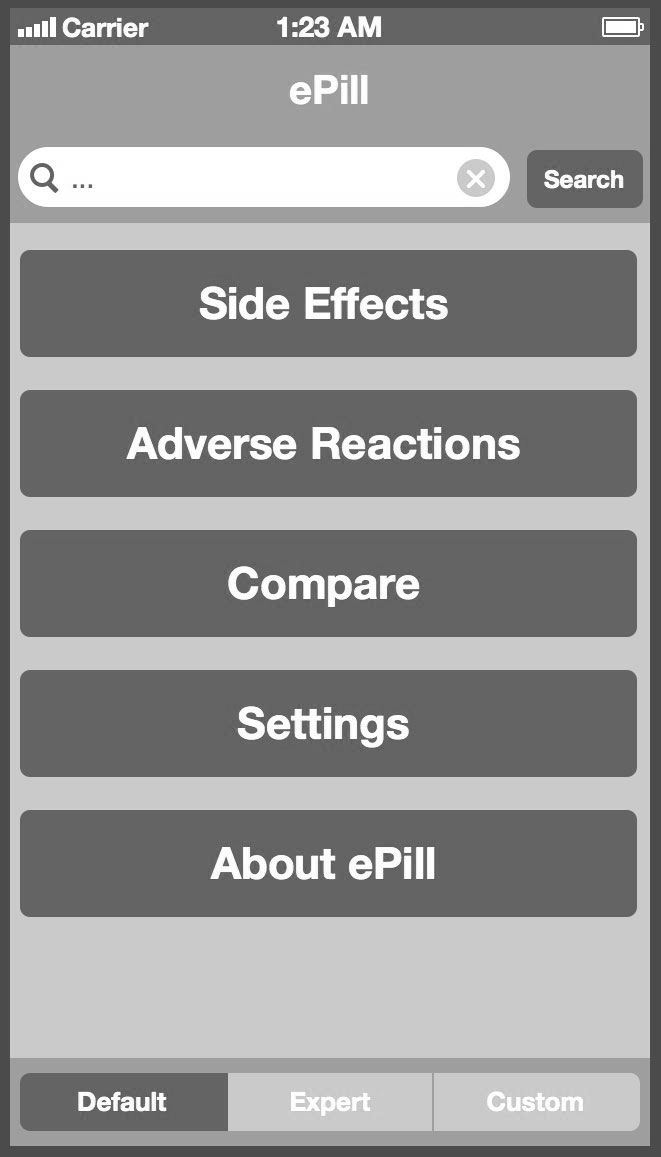
\includegraphics[width=0.8025\linewidth]{figures/Screen_1_bw.jpg}
        \caption[Main Screen Mockup]{Main Screen Mockup}
        \label{fig:Mockup}

    \end{minipage}
    \hspace{0.5cm}
    \begin{minipage}[b]{0.45\linewidth}
        \centering
        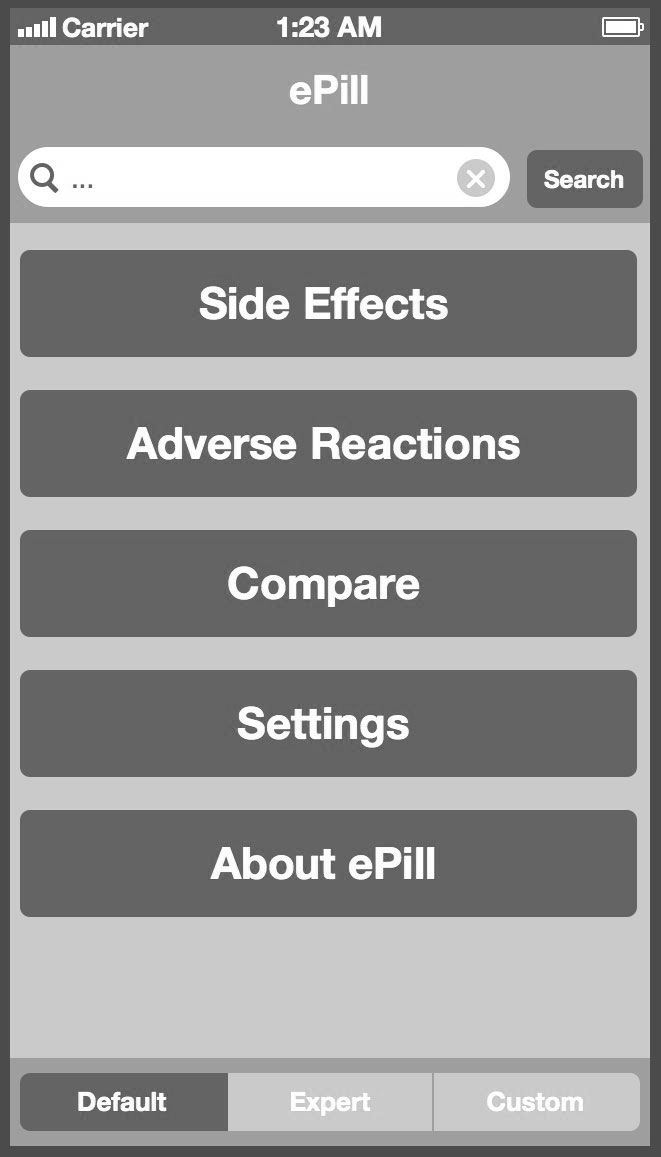
\includegraphics[width=0.8025\linewidth]{figures/Screen_1_bw.jpg}
        \caption[Final Main Screen]{Final Main Screen}
        \label{fig:FinalMainScreen}

    \end{minipage}
    \\
    \\
    \\
    \begin{minipage}[b]{0.45\linewidth}
        \centering
        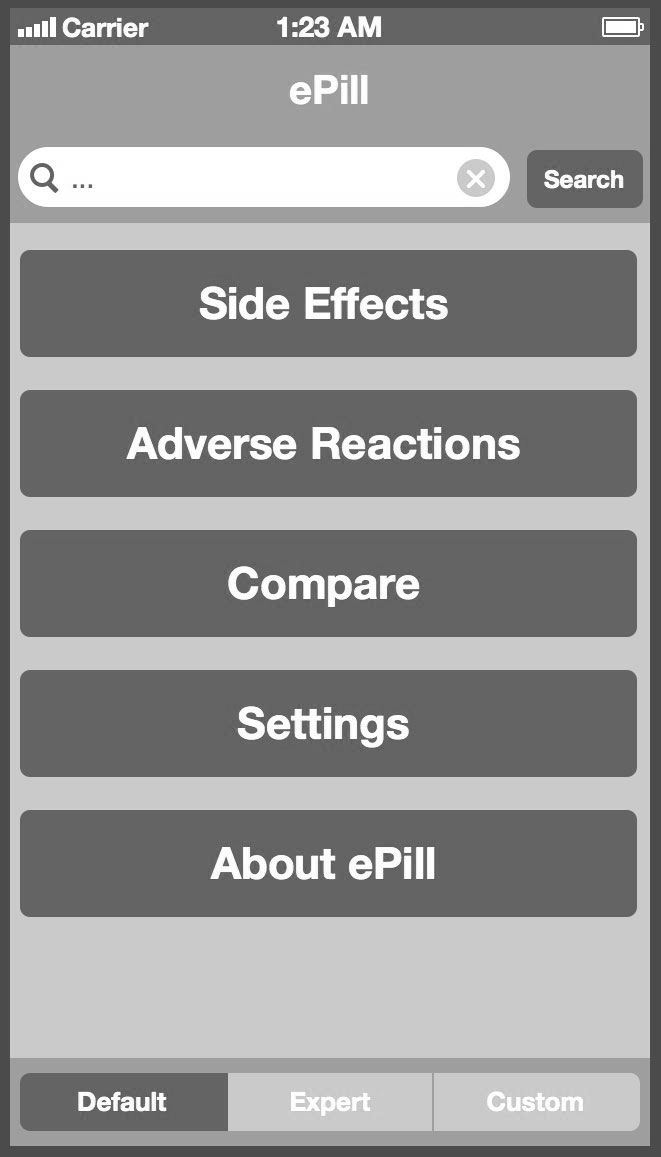
\includegraphics[width=0.8025\linewidth]{figures/Screen_1_bw.jpg}
        \caption[Search Input Screen]{Search Input Screen}
        \label{fig:SearchInputScreen}

    \end{minipage}
    \hspace{0.5cm}
    \begin{minipage}[b]{0.45\linewidth}
        \centering
        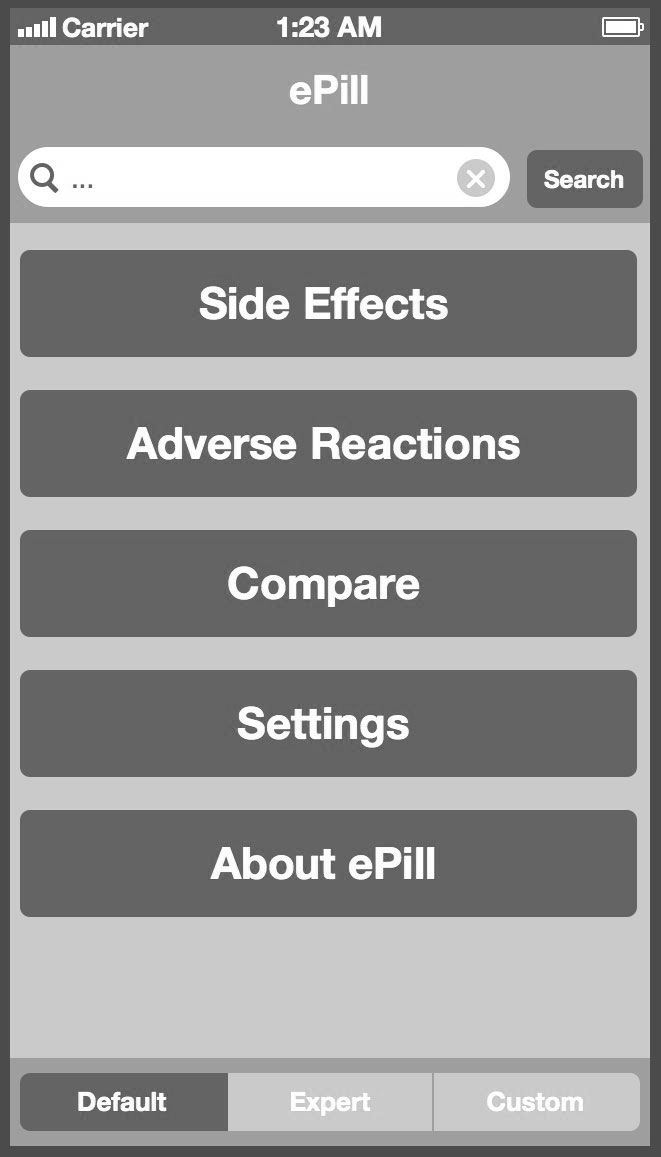
\includegraphics[width=0.8025\linewidth]{figures/Screen_1_bw.jpg}
        \caption[Search Result Screen]{Search Result Screen}
        \label{fig:SearchResultScreen}

    \end{minipage}
\end{figure}
\\
The three major functions of ePill (Search, Display and Supplementing Services) should be accessible as fast as possible. Of course, the display functionality and some supplementing services (e.g. the term explanation functionality) are only able to present results, if a pharmaceutical is selected. So we designed \ref{fig:Mockup} as a stripped down starting screen with every main function quickly available. Due to some missing generic controls provided by Vaadin TouchKit, like the search bar, we finally implemented the start screen as illustrated in \ref{fig:FinalMainScreen}. This resulted furthermore in a more separated presentation of search string input view and result view, as presented in \ref{fig:SearchInputScreen} and \ref{fig:SearchResultScreen}.
\\
\\
Throughout the planning and designing we tried to reproduce common patterns and user controls. Therefor we utilized the navigation back on the top left corner, illustrated by a leftwards oriented arrow-shaped button. Central navigation which specified the view, e.g. main function selection or the selection of a specific pharmaceutical from e.g. a search result list, is centered in the main content area in the screen's center.
\\
\\
Most of the views offer a toolbar at the screen's bottom. This toolbar contains controls which are used for navigation inside the screen's center view, e.g. go back to top or navigate to a specific header. Especially in the pharmaceutical details view with much information visible, it can be very handy to jump right to the header one is interested in. Additionally, some controls are added in the toolbar which enable further interaction with the information displayed, e.g. adding the currently visible pharmaceutical to the current list, which I will discuss later.
\\
\\
The web application has rich customization possibilities. One can adjust the font size, the details of pharmaceuticals to be displayed and the layout of the web application itself. As it turned out, it is not applicable for the user to change the mobile apps layout, because the user interface so too compact to add additional elements and too few elements are visible to hide any element.
\\
\\
The current list is a concept added to the mobile application and derived from a view in the web application. The web application offers a view in which pharmaceuticals can be added and afterwards, via a button click, aggregated information, like adverse reactions, can be listed. Because we have much less available screen space in the mobile app, we decided to have the list globally available throughout the entire app. E.g. if one searched for a pharmaceutical and has selected one to display detailed information, one can easily via a button in the toolbar add this pharmaceutical to one's current list. If one now selects e.g. the side effects functionality in the main screen, one sees his current list and can add more to it. This screen is illustrated in \ref{fig:CurrentListScreen}. If one decides to do so, one is presented a search input screen but can in the search result screen only tick on those pharmaceuticals one wants to add to one's current list and not see the pharmaceutical details on click. This is illustrated in \ref{fig:AlternativeListScreen}.
\begin{figure}[!tb]
    \begin{minipage}[b]{0.45\linewidth}
        \centering
        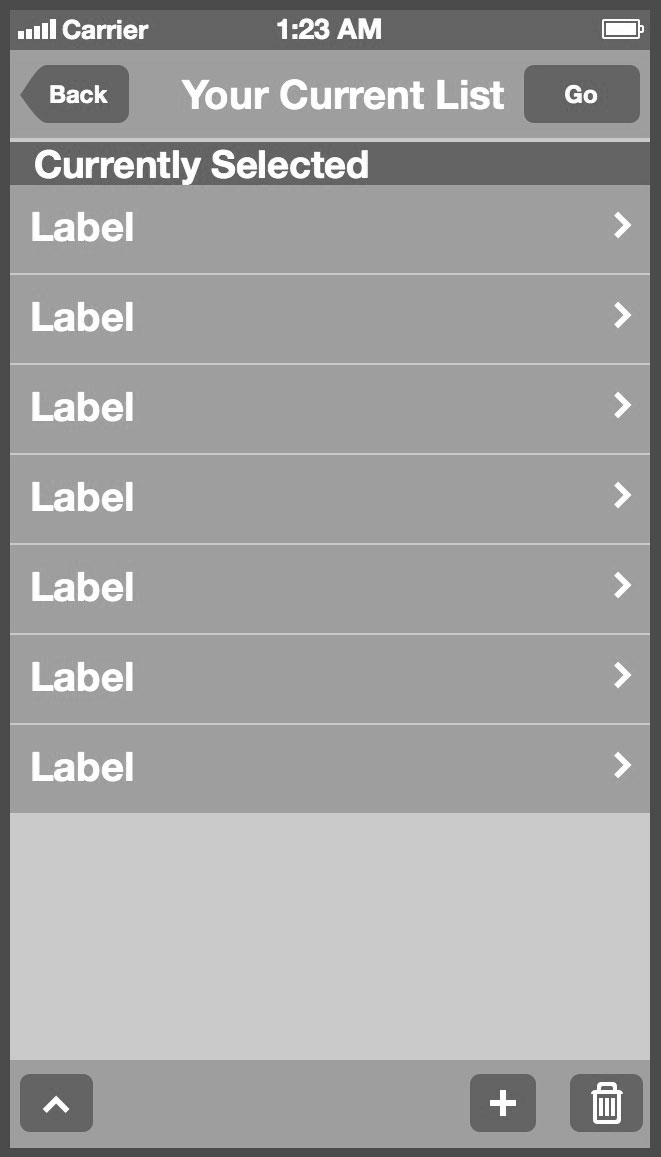
\includegraphics[width=0.8025\linewidth]{figures/Screen_2_bw.jpg}
        \caption[Current List Screen]{Current List Screen}
        \label{fig:CurrentListScreen}

    \end{minipage}
    \hspace{0.5cm}
    \begin{minipage}[b]{0.45\linewidth}
        \centering
        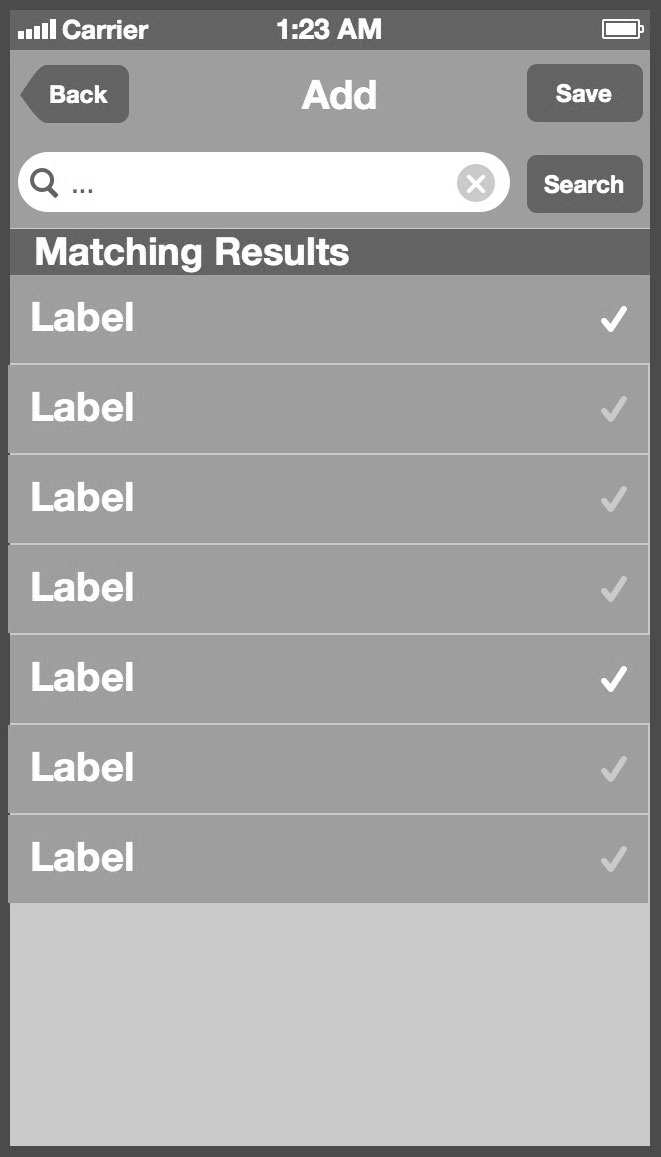
\includegraphics[width=0.8025\linewidth]{figures/Screen_3_bw.jpg}
        \caption[List Screen to add to Current List]{Alternative List Screen}
        \label{fig:AlternativeListScreen}

    \end{minipage}
\end{figure}

\subsection{The Implementation Process}
\label{subsec:Implementation}

\subsection{Validation of the mobile App}
\label{subsec:Validation}